

\begin{figure}
		\begin{subfigure}{.5\textwidth}
		  \centering
		  	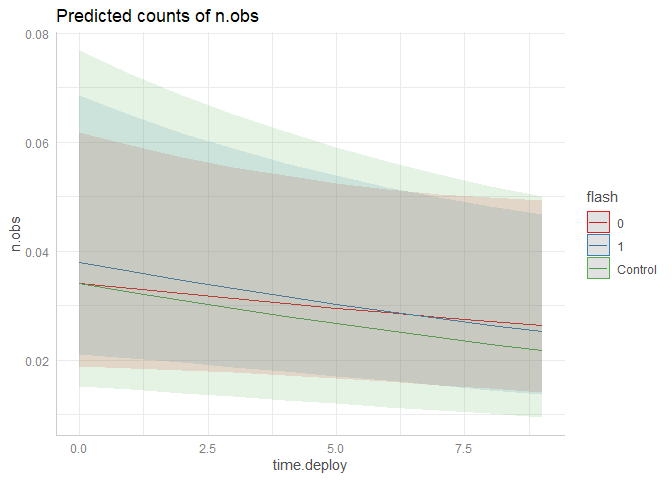
\includegraphics[width=.8\linewidth]{../R/glmm_sp_files/figure-gfm/raadyr-C-report-1.png}
		  \caption{Roe deer}
		  	\label{fig:glmm_raa}
	\end{subfigure}
		\begin{subfigure}{.5\textwidth}
		  \centering
		  	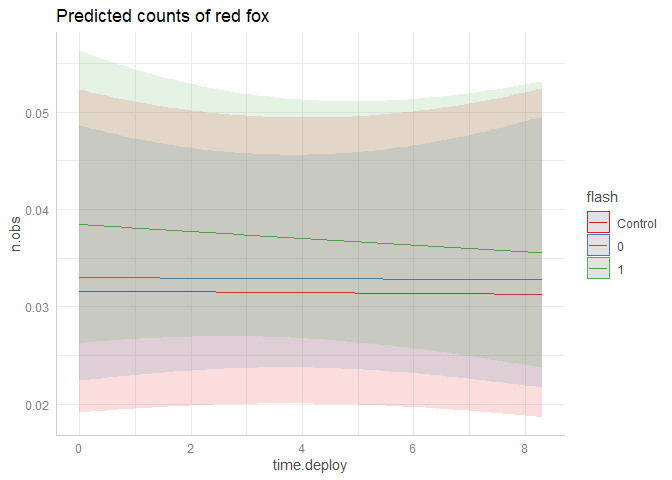
\includegraphics[width=.8\linewidth]{../R/glmm_sp_files/figure-gfm/rev-report-1.png}
		  \caption{Red fox}
		  	\label{fig:glmm_rev}
	\end{subfigure}
		\begin{subfigure}{.5\textwidth}
		  \centering
		  	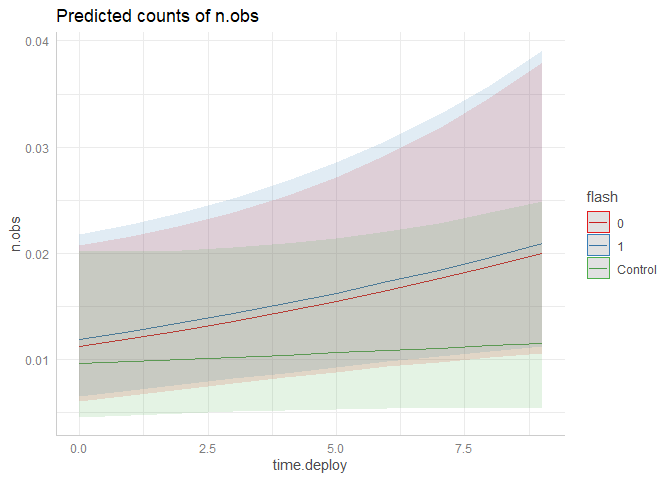
\includegraphics[width=.8\linewidth]{../R/glmm_sp_files/figure-gfm/grevling-report-1.png}
		  \caption{Badger}
		  	\label{fig:glmm_grvl}
	\end{subfigure}
		\begin{subfigure}{.5\textwidth}
		  \centering
		  	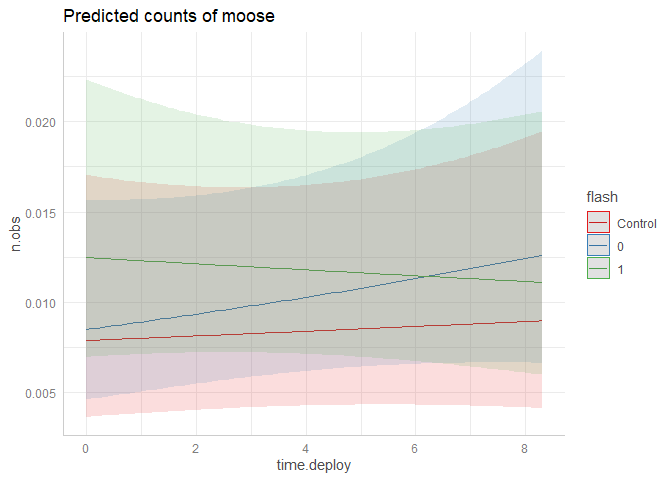
\includegraphics[width=.8\linewidth]{../R/glmm_sp_files/figure-gfm/elg-report-1.png}
		  \caption{Moose}
		  	\label{fig:glmm_elg}
	\end{subfigure}
		\begin{subfigure}{.5\textwidth}
		  \centering
		  	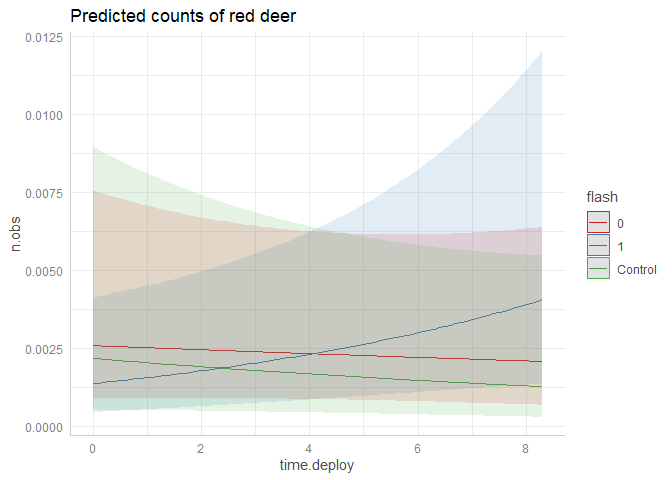
\includegraphics[width=.8\linewidth]{../R/glmm_sp_files/figure-gfm/hjort-report-1.png}
		  \caption{Red deer}
		  	\label{fig:glmm_hjort}
	\end{subfigure}
		\begin{subfigure}{.5\textwidth}
		  \centering
		  	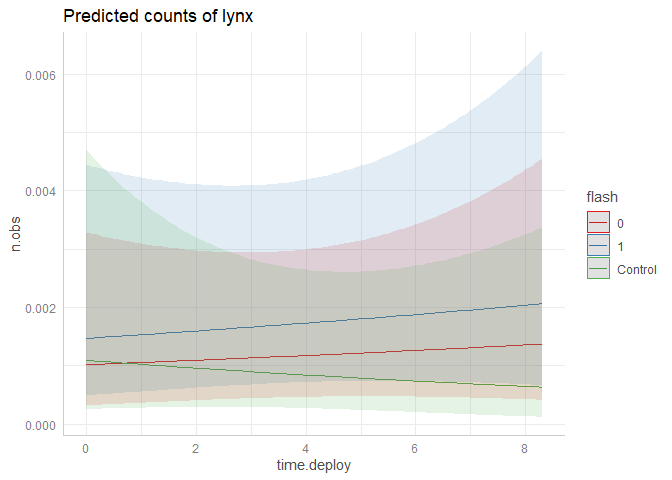
\includegraphics[width=.8\linewidth]{../R/glmm_sp_files/figure-gfm/gaupe-report-1.png}
		  \caption{Lynx}
		  	\label{fig:glmm_gaup}
	\end{subfigure}
		\caption{Fitted GLMM model to each species}
	\label{fig:glmm_sp}
\end{figure}



\begin{figure}
		\begin{subfigure}{.4\textwidth}
		  \centering
	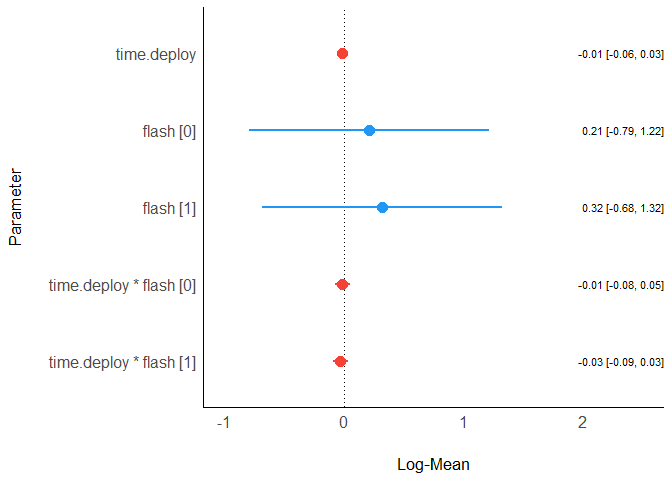
\includegraphics[scale=.4]{../R/glmm_sp_files/figure-gfm/parameters-1.png}
\caption{Intercept included}
		\label{fig:para_raa1}
	\end{subfigure}
		\begin{subfigure}{.4\textwidth}
		  \centering
	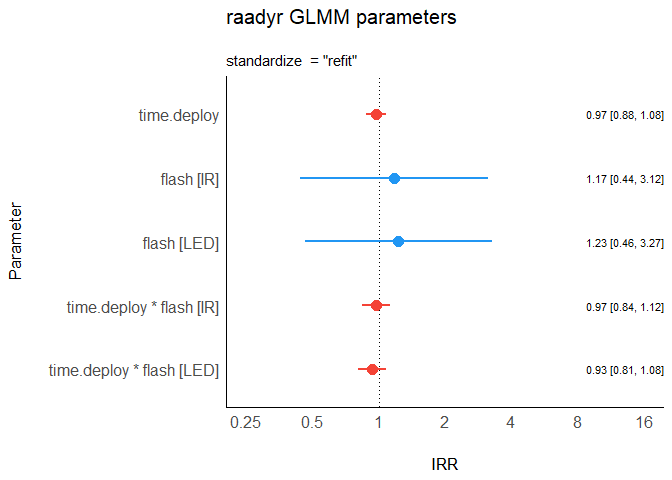
\includegraphics[scale=.4]{../R/glmm_sp_files/figure-gfm/parameters-2.png}
\caption{with values printed}
		\label{fig:para_raa2}
	\end{subfigure}
		\begin{subfigure}{.8\textwidth}
		  \centering
	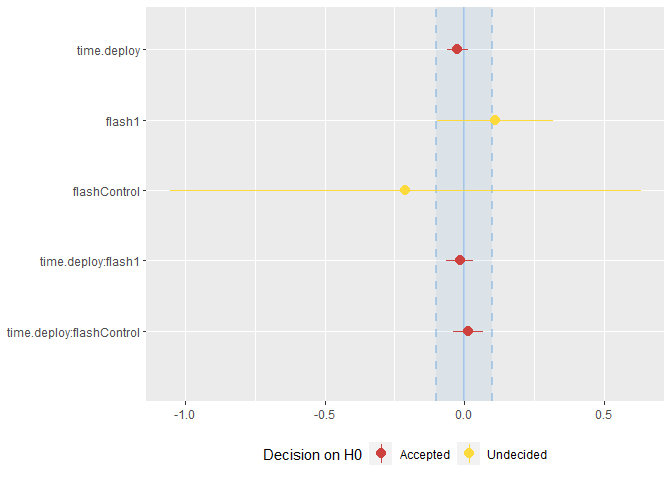
\includegraphics[scale=1]{../R/glmm_sp_files/figure-gfm/parameters-3.png}
\caption{Equivalence test}
		\label{fig:para_raa3}
	\end{subfigure}
		\caption{Visualising model parameters}
	\label{fig:para_sp}
\end{figure}

